%! TeX program = lualatex
\documentclass[../main.tex]{subfiles}
\begin{document} \section{Vector Fields}\label{sec:linalg-vector-fields}

A vector field is a function that takes \(n\)-dimensional vectors as inputs and outputs \(n\)-dimensional vectors. For the rest of the course, we are going to use a particular class of vector fields called a linear vector field.

TODO: Start the lecture with a wind map. 

\begin{definition}[linear vector field]
  A \hlmain{linear vector field} is defined square matrix.  In other words, given a square matrix \(A\), we can define a linear vector field \(\vec{F}\) by
  \[
    F(\vec{x}) = A \vec{x}.
  \]

  Conversely, if we know \(\vec{F}\) is a linear vector field, then there must be a square matrix \(A\) so that \(\vec{F}(\vec{x}) = A \vec{x}\).
\end{definition}

Linear vector fields are immensely useful because their pictorial representation can be used to encodes changes over time.  We introduce their visualization through an example.

\begin{example} \label{ex:linear-vector-field-intro}
  Perform the following calculations.
  \[
    \begin{bmatrix}
      0 & -0.1 \\
      0.2 & 0
    \end{bmatrix}
    \begin{bmatrix}
      3 \\ 2
    \end{bmatrix}
    =
    \begin{bmatrix}
      \phantom{-0.4} \\ \phantom{0.3}
    \end{bmatrix}
    ,\qquad
    \begin{bmatrix}
      0 & -0.1 \\
      0.2 & 0
    \end{bmatrix}
    \begin{bmatrix}
      -2 \\ 3
    \end{bmatrix}
    =
    \begin{bmatrix}
      \phantom{-0.6} \\ \phantom{-0.2}
    \end{bmatrix}
    ,\qquad
    \begin{bmatrix}
      0 & -0.1 \\
      0.2 & 0
    \end{bmatrix}
    \begin{bmatrix}
      -1 \\ -4
    \end{bmatrix}
    =
    \begin{bmatrix}
      \phantom{0.8} \\ \phantom{-0.1}
    \end{bmatrix}.
  \]
  \blanklines{10}

  Plot each input to the vector field as a point and its outputs as a vector coming out of the input dot. 

  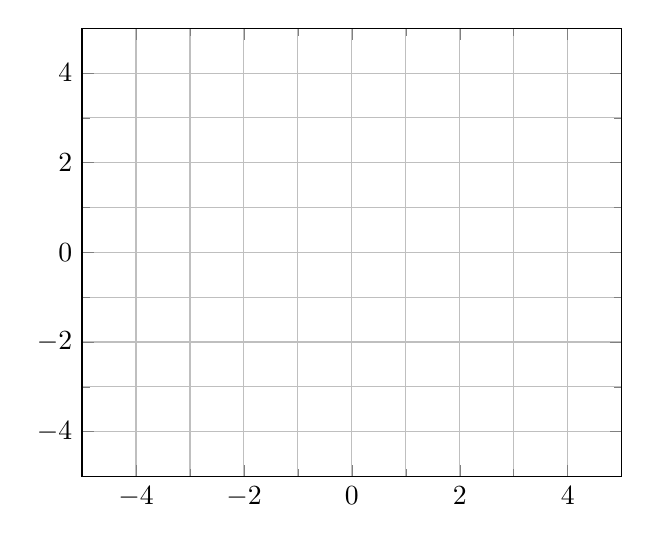
\begin{tikzpicture}[scale=1]
    \begin{axis}[xmin=-5, xmax=5, ymin=-5, ymax=5, minor tick num=1, grid=both]
    \end{axis}
  \end{tikzpicture}
\end{example}
\clearpage

Example~\ref{ex:linear-vector-field-intro} \emph{suggests} that we can \emph{interpret} interpret dots as \hlmain{states} and the arrow coming out of a dot as \hlmain{change}. 

\begin{example}
  Let \(A = \begin{bmatrix} 0 & -0.1 \\ 0.2 & 0 \end{bmatrix}\) be the matrix in Example~\ref{ex:linear-vector-field-intro}.  Let \(v = \begin{bmatrix} 3 \\ 2 \end{bmatrix}\). 

  Perform the following calculations.
  \[
    A \vec{v} = \hspace{1in}, \qquad
    A (A \vec{v}) = \hspace{1in}, \qquad
    A (A (A \vec{v})) = \hspace{1in}.
  \]
  \blanklines{10}

  Plot each input to the vector field as a point and its outputs as a vector coming out of the input dot. 

  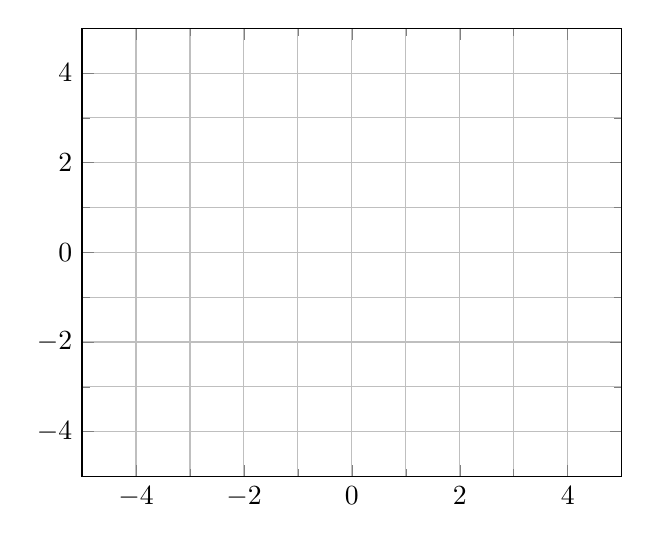
\begin{tikzpicture}[scale=1]
    \begin{axis}[xmin=-5, xmax=5, ymin=-5, ymax=5, minor tick num=1, grid=both]
    \end{axis}
  \end{tikzpicture}
\end{example}

\begin{example}[Example~6 on page 157 of the textbook]
  Consider a population of juveniles and adults.  At the end of each year, 
  \begin{itemize}
    \item \(20\%\) of the surviving juveniles become adults, 
    \item \(90\%\) of the adults survive, and
    \item the per-adult-capita birth rate is \(15\%\). 
  \end{itemize}

  Encode the age-structured population dynamics as a vector field and predict the number of adults and juveniles after \(2\) years if the initial population consists of \(2\) juveniles and \(4\) adults.

  \blanklines{5}
\end{example}
\end{document}
